\documentclass[11pt]{article}
\input{/Users/markwang/.preamble}
\begin{document}




% arg1=pdfurl arg2=pagenum arg3=sectiontitle
\newcommand{\linksection}[3][../../bishop_pattern_recognition_and_machine_learning.pdf]{
    \subsection*{\href[page=#2]{#1}{#3}}
}

\newcommand{\linkinline}[3][../../bishop_pattern_recognition_and_machine_learning.pdf]{
    \noindent\href[page=#2]{#1}{#3}
}

\renewcommand{\norm}[1]{\left\lVert#1\right\rVert}
\renewcommand{\E}[2][]{\mathbb{E}_{#1}\left\{#2\right\}}
\newcommand{\var}[1]{var\{#1\}}
\newcommand{\cov}[1]{cov\{#1\}} 
\newcommand{\normal}[1]{\mathcal{N}\left(#1\right)}
\newcommand{\exponents}[1]{exp\left\{#1\right\}}

\newcommand{\bmu}{\boldsymbol{\mu}}
\newcommand{\bpi}{\boldsymbol{\pi}}
\newcommand{\bTheta}{\boldsymbol{\Theta}}
\newcommand{\bSigma}{\boldsymbol{\Sigma}}
\newcommand{\bphi}{\boldsymbol{\phi}}


\newcommand{\calR}{\mathcal{R}}
\newcommand{\calC}{\mathcal{C}}
\newcommand{\calD}{\mathcal{D}}
\newcommand{\bx}{\matr{x}}
\newcommand{\bt}{\matr{t}}
\newcommand{\bw}{\matr{w}}
\newcommand{\bX}{\matr{X}}
\newcommand{\bZ}{\matr{Z}}
\newcommand{\bz}{\matr{z}}


\newcommand{\lebpar}[2]{\frac{\partial #1}{\partial #2}}
\newcommand{\qqqquad}{\quad \quad \quad \quad}




\linksection{439}{9 Mixture Models and EM}
\linksection{440}{9.1 K-means Clustering}

\begin{defn*}
    \textbf{Concepts}
    \begin{enumerate}
        \item \textbf{Clustering} 
        \item \textbf{K-means} Problem with K-means is that at every step, every point is assigned to one and only one cluster centers, but maybe many points which are halfway between cluster centers. It is beneficial to have soft assignment of such points by adopting a probabilistic viewpoint
        \item \textbf{Application} in image segmentation and compression
    \end{enumerate}
\end{defn*}


\linksection{446}{9.2 Mixture of Gaussians}

\begin{defn*}
    \textbf{Mixtures of Gaussians} Given 
    \[
        p(\bx) = \sum_{k=1}^K \pi_k \normal{\bx | \bmu_k, \boldsymbol{\Sigma}_k}    
    \]
    Reformulate linear mixture models as Gaussian mixtures in terms of discrete latent variables. Goal is to define random variable $\bx$ and $\bz$ such that the distribution of $\bx$ is equivalent to linear basis model with Gaussian kernel 
    \[
        p(\bx)
        = \sum_{\bz} p(\bx,\bz)
        = \sum_{\bz} p(\bx | \bz) p(\bz)
    \]
    Define $\bz: \text{1-of-K encoding} \rightarrow [0,1]$ as a soft assignment to cluster centers. then marginal distribution over $\bz$ given by 
    \[
        p(\bz) = \prod_{k=1}^K \pi_k^{z_k}
        \qquad \text{such that} \qquad 
        p(z_k) = \pi_k    
    \] 
    Define conditional distribution of $\bx$ over $\bz$ as Gaussian 
    \[
        p(\bx | \bz) = \prod_{k=1}^K \normal{\bx | \bmu_k, \bSigma}^{z_k}    
        \qquad \text{such that} \qquad 
        p(\bx | z_k = 1) = \normal{\bx | \bmu_k, \bSigma_k}
    \]
    Therefore 
    \[
        p(\bx) = \sum_{\bz} p(\bx | \bz) p(\bz)
        = \sum_{k=1}^K \pi_k \normal{\bx | \bmu_k, \boldsymbol{\Sigma}_k}   
    \]
    The posterior distribution of $\bz$ given observation $\bx$, \textit{responsibility}, is given by 
    \[
        \gamma(z_k)\equiv p(z_k=1|\bx)
        = \frac{\pi_k \normal{\bx | \bmu_k, \bSigma_k}}{\sum_{k=1}^K \pi_j \normal{\bx | \bmu_j, \bSigma_j}}
    \]
    \begin{center}
        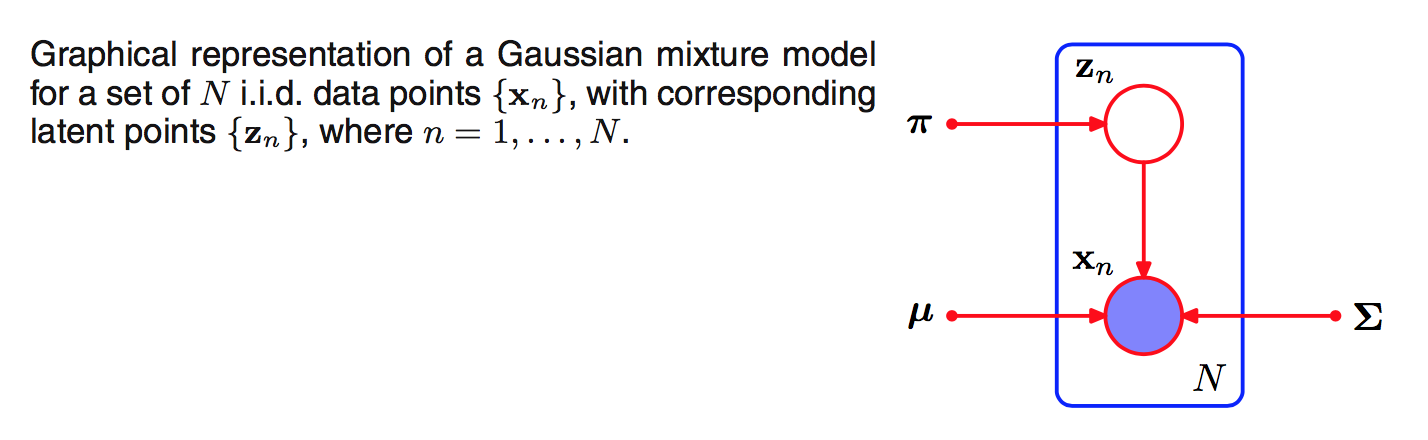
\includegraphics[width=10cm]{gaussian_mixture_graphical_model.png}
    \end{center}
\end{defn*}

\begin{defn*}
    \textbf{MLE for Gaussian Mixtures} \\
    Assume $N\times D$ matrix $\bX = \{\bx_i\}_{i=1}^N$ and $N\times K$ matrix $\bZ = \{ \bz_i \}_{i=1}^N$, then we want to maximize log likelihood
    \[
        \ln p(\bX | \bpi, \bmu, \bSigma) 
        = \ln \prod_{n=1}^N p(\bx_n)
        = \sum_{n=1}^N \ln \left\{ 
            \sum_{k=1}^K \pi_k \normal{\bx_n | \bmu_k, \bSigma_k}
             \right\}
    \]
    Maximum likelihood has some problems (\linkinline{450}{here})
    \begin{enumerate}
        \item overfits because of existence of \textit
        {singularity}
        \item \textit{identifiability} problem
    \end{enumerate}
    Naively, we solve MLE by taking derivative with respect to $\bmu$, $\bSigma$, and $\bpi$, the solution is not a closed form solution as $N_k$ invovles parameters that we want to estimate
    \[
        \bmu_k = \frac{1}{N_k} \sum_{n=1}^K \gamma(z_{nk}) \bx_n
        \qquad 
        \bSigma_k = \frac{1}{N_k}\sum_{n=1}^N \gamma(z_{nk}) \norm{\bx_n - \bmu_k}^2
        \qquad 
        \pi_k = \frac{N_k}{N}
    \]
    where $N_k = \textstyle \sum_{n=1}^N \gamma(r_{nk})$ represents the \textbf{ effective number of points} assigned to cluster $k$. MLE estimator $\bmu_k$ for $k$-th Gaussian component is obtained by taking a weighted mean of all points in the dataset in which the weight factor for each data point $\bx_n$ is given by the posterior probability $\gamma(z_{nk}) = p(z_{nk}=1|\bX)$ tha component $k$ was responsible for generating $\bx_n$. $\pi_k$ the $k$-th \textbf{mixing coefficient} is given by the average responsibility that component takes for explaining the dataset
\end{defn*}  

\begin{defn*}
    \textbf{EM for Gaussian Mixtures} \\
    The goal is to maximize the likelihood function $p(\bX | \bpi, \bmu, \bSigma)$ for which there is no closed form solution. (detailed \linkinline{455}{here})
    \begin{enumerate}
        \item Pick some initial value for $\bmu, \bSigma, \bpi$, and alternate between E step and M step
        \item \textbf{E step} use value of parameter to evaluate the responsibility $\gamma(r_{nk})$, i.e. soft assignment
        \item \textbf{M step} re-estimate $\bmu, \bSigma, \bpi$ using maximum likelihood formulas
        \item Evaluate log likelihood by 
        \[
            \ln p(\bX | \bpi, \bmu, \bSigma)
            = \sum_{n=1}^N \ln \left\{ 
                \sum_{k=1}^K \pi_k \normal{\bx_n | \bmu_k, \bSigma_k}
                 \right\}
        \]
        check for convergence, return to step 2 if convergence criterion not satisfied
    \end{enumerate}
\end{defn*}


\linksection{455}{9.3 An alternative view of EM}

\begin{defn*}
    \textbf{Expectation-Maximization}
    \begin{enumerate}
        \item \textbf{Goal}: find maximum likelihood solutions for models having latent variables
        \item \textbf{EM model} Given observed data $\bX$ and latent variables $\bZ$, and set of model parameters $\bTheta$, we want to maximize the log likelihood function 
        \[
            \ln p(\bX | \bTheta) = 
            \ln \left\{ \sum_{\bZ} p(\bX, \bZ | \bTheta) \right\}    
        \]
        $\{\bX, \bZ\}$ is the commplete dataset, and he actual observed $\{\bX\}$ is incomplete dataset. 
        \item \textbf{EM algorithm sketch} Idea is we cannot compute complete-data likelihood $\ln p(\bX,\bZ | \bTheta)$ but we instead approximate it with posterior of latent variable $p(\bZ | \bX, \bTheta)$ (E step). The expectation is given by 
        \[
            \mathcal{Q}(\bTheta, \bTheta^{old})
            = \E[\bZ \sim p(\bZ | \bX,\bTheta^{old})]{\ln p(\bX, \bZ | \bTheta)}
            = \sum_{\bZ} p(\bZ | \bX, \bTheta^{old}) \ln p(\bX, \bZ | \bTheta)
        \]
        Then we maximize this expectation with respect to the parameters (M step).
        \[
            \bTheta^{new}
            = \argmax_{\bTheta}  \mathcal{Q}(\bTheta, \bTheta^{old})
        \]
        Detailed algorithm \linkinline{457}{here}
    \end{enumerate}
\end{defn*}



\begin{defn*}
    \textbf{Gaussian Mixture Revisited} \\ 
    If given complete data $\{\bX, \bZ\}$, then the graphical model is as follows
    \begin{center}
        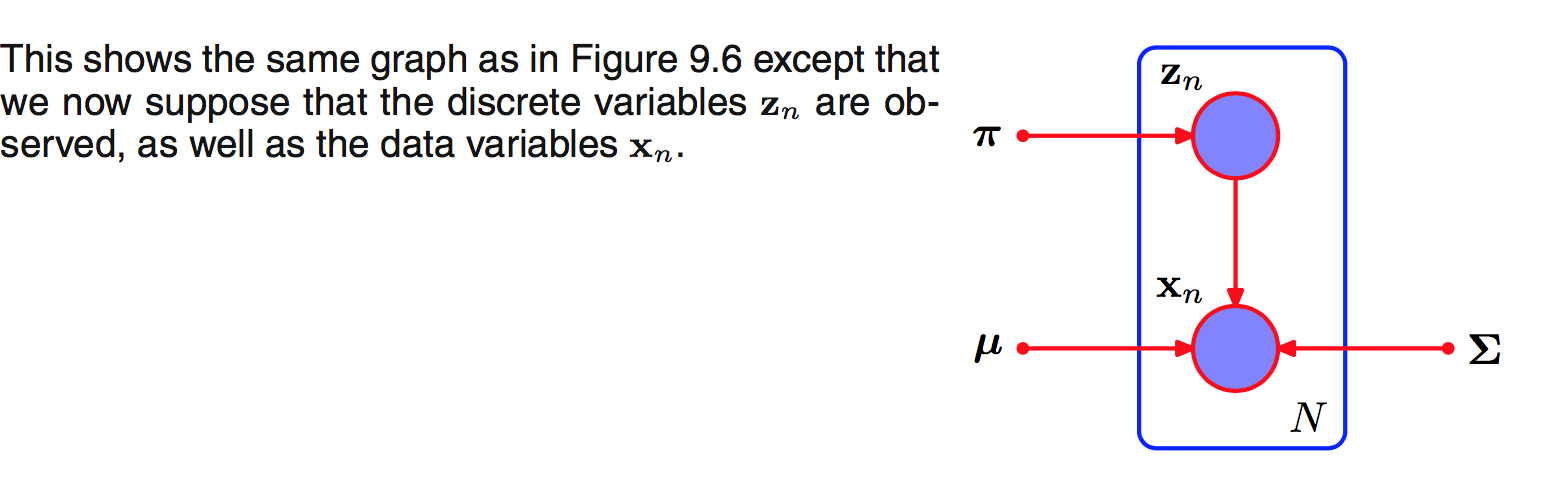
\includegraphics[width=10cm]{gaussian_mixture_graphical_model_completedata.png}
    \end{center}
    the likelihood function is simply the joint distribution of $\bX, \bZ$ over deterministic model parameters
    \[
        p(\bX, \bZ | \bmu, \bSigma, \bpi)
        \overset{graphical}{=} \prod_{n=1}^N p(\bx_n | \bz_n ) p(\bz_n)
        = \prod_{n=1}^N \prod_{k=1}^K \pi_k^{z_{nk}} \normal{\bx_n | \bmu_k, \bSigma_k}^{z_{nk}}
    \]
    Note this is different from previous log likelihood where only have incomplete data $\{\bX \}$ in that we have to consider joint distribution of both $\bX$ and $\bZ$ since both are observed variables. We note that this likelihood fucntion have closed form solution and so EM algorithm works trivially
    \[
        \mathcal{L}_{complete} 
        = \ln  p(\bX, \bZ | \bmu, \bSigma, \bpi)
        = \sum_n \sum_k z_{nk} 
        \left( 
            \ln \pi_k + \ln \normal{\bx_n | \bmu_k, \bSigma_k}    
        \right)
    \]
    If give only incomplete data $\{\bX\}$, then using Bayes rule to get posterior distribution of $\bZ$ 
    \[
        p(\bZ | \bX, \bmu, \bSigma, \bpi) 
        \propto p(\bZ, \bX)
        = \prod_{n=1}^N \prod_{k=1}^K \left( \pi_k \normal{\bx_n | \bmu_k, \bSigma_k} \right)^{z_{nk}}
    \]
    where $\{\bz_n \}$ are independent in this case. Then we can derive expectation that we want to maximize 
    \[
        \mathcal{L}_{incomplete}
        = \E[\bZ]{p(\bZ | \bX, \bmu, \bSigma, \bpi)}
        = \sum_{n=1}^N \sum_{k=1}^K \gamma(z_{nk})(\ln \pi_k + \ln \normal{\bx_n | \bmu_k, \bSigma_k})
    \]
    which has no closed form solution, so we use EM algorithm exactly the same as before.
\end{defn*}


\begin{defn*}
    \textbf{Relation to K-means} \\
    \begin{enumerate}
        \item \textbf{Comparison} K-means performs \textbf{hard assignment} of data potins to clusters. The EM algorithm makes \textbf{soft assignment} based on posterior probabilities
        \item \textbf{Idea} A Gaussian mixture model in which covariance matrix are given by $\epsilon I$ where $\epsilon \rightarrow 0$ is equivalent to K-means, i.e. 
        \[
            \gamma(z_{nk}) \overset{\epsilon \rightarrow 0}{\longrightarrow} r_{nk}
        \]
        \[
            \E[\bZ]{\ln p(\bX, \bZ | \bmu, \bSigma, \bpi)} \overset{\epsilon\rightarrow 0}{\longrightarrow}
            - \sum_n \sum_k r_{nk} \norm{\bx_n - \bmu_k}^2
        \]
        Also note that K-means does not estimate covariances of clusters but only cluster means. 
    \end{enumerate}
\end{defn*}


\end{document}
 